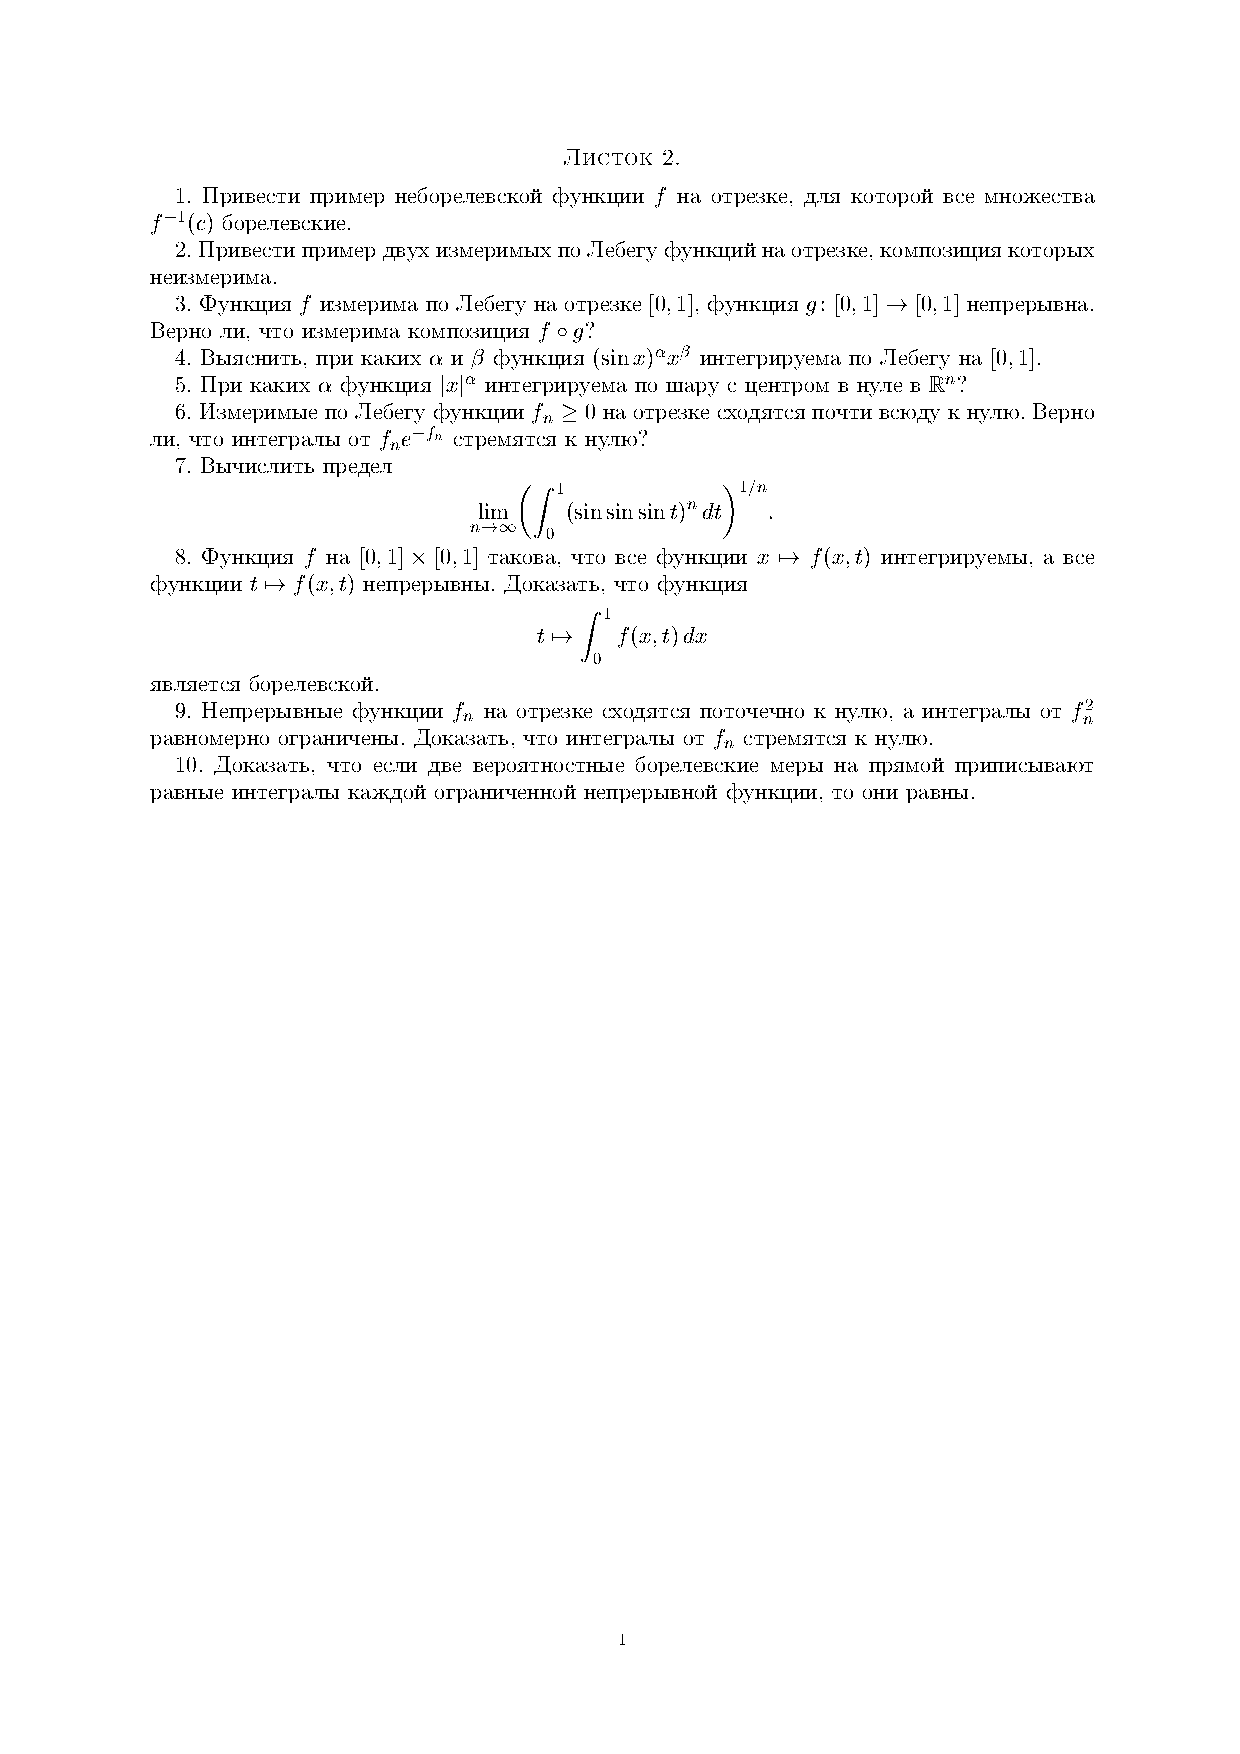
\includepdf[scale=0.95,pages=1,pagecommand=\section*{Условия}]{Tasks/listok-matan2}
\newpage
\section*{Решения}
\subsection*{Задача 1}
	Рассмотрим $f: [0,1] \to [0,2]$ и 
	\begin{gather*}
		f(x) =
		\begin{cases}
			x\quad x \in V\\
			x+1\quad x \notin V
		\end{cases}
	\end{gather*}
	Где $V$ -- множество Витали, тогда
	\begin{gather*}
		f(c) =
		\begin{cases}
			c\quad c \in V\\
			c-1\quad c \notin V
		\end{cases}
	\end{gather*}
	И $f^{-1}(c)$ борелевское множество\\
	$f(x)$ измерима относительно $B(\mathbb{R})$, если $f^{-1}(B) \in B(\mathbb{R})$ для любого борелевского $B$\\
	При $B = [0,1],\ f^{-1}(B) = V$, следовательно $f$ -- неборелевская функция
	\vskip0.5in


\subsection*{Задача 2}
	Пусть $\varphi(x)$ -- Канторова лестница, $\psi(x) = \frac{1}{2} (\varphi(x) + x),\ \psi:[0,1] \to [0,1]$ -- взаимно однозначная функция, непрерывна и монотонно возрастает, следовательно она измерима по Лебегу и существует обратное отображение с такими же свойствами, а $K$ -- Канторово множество.
	\begin{gather*}
		\mu(K) = 0,\ \mu([0,1]\backslash K) = 1\\
		\mu(\psi([a_1,a_2])) = \mu \left(\frac{\varphi(a_1,a_2) + (a_1,a_2)}{2}\right) = \mu \left(\frac{(a_1,a_2)}{2}\right)\\
		\mu(\psi(K)) = \mu(\psi([0,1])) - \mu(\psi([0,1]\backslash K)) = 1 - \frac{1}{2} = \frac{1}{2}
	\end{gather*}
	Так как $\mu(\psi(K)) \ne 0$, то существует неизмеримое множество $M \subset \psi(K)$
	\begin{gather*}
		\psi^{-1}(M) \subset K\\
		\mu(K) = 0
	\end{gather*}
	Следовательно $\psi^{-1}(M)$ измеримо по Лебегу\\
	Пусть $N = \psi^{-1}(M)$, тогда рассмотрим $I_N (\psi^{-1}(x))$, оно неизмеримо, так как $(I_N \circ \psi^{-1})(1) = \psi(I_N^{-1}(1)) = \psi(N) = M$ -- неизмеримо
	\vskip0.5in
\begin{comment}
	Пусть $f: [0,1] \to [0,1]$ -- Канторова лестница. На канторовом множестве $K$: $f(x) = \sup\limits_{\substack{y < x \\ y \notin K}} f(y)$, если $x \in K$. Тогда $f$ непрерывная.\\
	Пусть $g(x) = f(x) + x$, $g: [0,1] \to [0,2]$, $g$ непрерывна и монотонно возрастает.
	\begin{gather*}
	\mu(g(K)) = 1\\
	\mu(g(a_ia_j)) = l(a_i,a_j)\qquad a_i a_j\text{ -- некий отрезок, } l(a_i, a_j) \text{ -- его длина}\\
	\mu(g([0,1] \backslash K)) = \sum\limits_{i,j} \mu(g(a_i a_j)) = \sum\limits_{i,j} \mu(a_i a_j) = \mu(\sum a_i a_j) = \mu([0,1] \backslash K) = 1
	\end{gather*}
	Получается, что $\mu(g(K)) = \mu(g[0,1]) - \mu(g([0,1] \backslash K)) = 2 - 1 = 1$, тогда существует неизмеримое $M \subset g(K)$, так как в любом множестве ненулевой меры существует неизмеримое подмножество.\\
	$N = g^{-1}(M)$, рассмотрим композицию $I_N \circ g^{-1}$. Заметим, что $g^{-1}$ измерима, так как непрерывна.\\
	$N \subset K$, следовательно $\mu(N) = 0$, следовательно $I_N$ измерима.\\
	$I_N \circ g^{-1}$ неизмерима, так как $(I_n \circ g^{-1})^{-1} (1) = (g \circ I_n^{-1})(1) = g(N) = M$ -- неизмерима, а $\{1\}$ -- борелевское множество, а для любого борелевского множества прообраз должен быть измерим, если функция измерима
\end{comment}
	
	
\subsection*{Задача 3}
	Неверно. Пусть $f(x)$ -- Канторова лестница, измерима по Лебегу на $[0,1]$, $g(x) = \frac{1}{2}(f(x) + x),\ g:[0,1] \to [0,1]$ -- непрерывна и монотонно возрастает, тогда $f \circ g$ неизмерима по 2 задаче.
	\vskip0.5in
	
	
\subsection*{Задача 4}
	Необходимо и достаточно показать сходимость интеграла как несобственного интеграла Римана $\int_{0}^{\varepsilon} x^{\beta} (\sin x)^{\alpha} + \int_{\varepsilon}^{1} x^{\beta} (\sin x)^{\alpha}\quad \forall \varepsilon \in [0,1]$ вторая часть интегрируема так как непрерывна. Тогда заметим, что $(\sin x)^{\alpha} x^{\beta} = \left(\frac{\sin x}{x}\right)^{\alpha} x^{\alpha + \beta}$ и $\lim\limits_{x \to 0} \frac{\sin x}{x} = 1$, поэтому необходим и достаточен факт того, что $x^{\alpha + \beta}$ интегрируема, а это выполнено при $\alpha + \beta > -1$
\begin{comment}
	$\sin x^{\alpha} = (x - \frac{x^3}{3!} + \frac{x^5}{5!} - \dots)^{\alpha} < x^{\alpha}$\\
	По определению, если ряд $\sum\limits_{n=1}^{\infty} \mu(x:\ |f(x)| \geqslant n)$ сходится, то $f$ интегрируема\\
	$(\sin x)^{\alpha} x^{\beta} < x^{\alpha + \beta}$\\
	Если ряд $\sum\limits_{n=1}^{\infty} \mu(x:\ x^{\alpha + \beta} \geqslant n)$ сходится, то ряд $\sum\limits_{n=1}^{\infty} \mu(x:\ (\sin x)^{\alpha} x^{\beta} \geqslant n)$ тоже сходится
	\begin{gather*}
	\sum\limits_{n=1}^{\infty} \mu(x:\ x^{\alpha + \beta} \geqslant n) = 
	\sum\limits_{n=1}^{\infty} \mu(x:\ x \geqslant n^{\frac{1}{\alpha + \beta}}) =
	\sum\limits_{n=1}^{\infty} n^{\frac{1}{\alpha + \beta}}
	\end{gather*}
	Сходится при $-\frac{1}{\alpha + \beta}\Leftrightarrow \alpha + \beta > -1$
\end{comment}
	\vskip0.5in


\subsection*{Задача 5}
	Заметим, что при $\alpha \geqslant 0,\ |x|^{\alpha}$ непрерывна и ограничена на шаре, поэтому интегрируема.\\
	$\int_{B_r(0)} |x|^{\alpha} d \mu$ существует $\leftrightarrow$ $\sum\limits_{n = 1}^{\infty} \mu(x:\ |x|^{\alpha} \geqslant n)$ сходится
	\begin{gather*}
		\sum\limits_{n=1}^{\infty} \mu(x: |x|^{\alpha} \geqslant n) =
		\sum\limits_{n=1}^{\infty} \mu(x: \frac{1}{|x|^{-\alpha}} \geqslant n) =
		\sum\limits_{n=1}^{\infty} \mu(x: |x|^{-\alpha} \leqslant \frac{1}{n}) =
		\sum\limits_{n=1}^{\infty} \mu(x: |x| \leqslant \left(\frac{1}{n}\right){-\frac{1}{\alpha}}) =
		\sum\limits_{n=1}^{\infty} \left(\frac{1}{n}\right)^{-\frac{k}{\alpha}} c
	\end{gather*}
	Так как объем шара радиуса $r$ это $r^{k} c$, где $c$ -- объем единичного шара\\
	То есть интегрируемость равносильна сходимости $\sum\limits_{n=1}^{\infty} \left(\frac{1}{n}\right)^{-\frac{k}{\alpha}}$, то есть $-\frac{k}{\alpha} > 1 \Leftrightarrow k > -\alpha$
	\vskip0.5in


\subsection*{Задача 6}
	Заметим, что $f_n \to 0$, $e^{f_n} \to 1$, следовательно $\frac{f_n}{e^{f_n}} \to 0$ почти всюду поточечно.\\
	Тогда заметим, что 
	\begin{gather*}
		\frac{f_n(x)}{e^{f_n(x)}} = \frac{f_n(x)}{1 + f_n(x) + \frac{f_n^{2}(x)}{2} + \dots} \leqslant \frac{f_n(x)}{f_n(x)} = 1
	\end{gather*}
	Функция $\Phi \cong 1$ интегрируема на отрезке, следовательно $\Phi$ -- интегрирующая мажоранта.\\
	По теореме Лебега о мажорированной сходимости $\lim\limits_{n \to \infty} \int_x f_n e^{-f_n} = 0$
	\vskip0.5in


\subsection*{Задача 7}
	\begin{gather*}
		\lim\limits_{n \to \infty}\left(\int_{0}^{1}(\sin\sin\sin t)^n dt \right)^{\frac{1}{n}}
	\end{gather*}
	Докажем, что $\lim\limits_{n \to \infty} ||f||_n = ||f||_{\infty}$ на $X: \mu(x) = 1$\\
	Для начала, покажем что $||f||_p$ возрастает, запишем неравенство Гельдера:
	\begin{gather*}
		\int_{x} |fg| d\mu \leqslant (\int_{x} |f|^p d \mu)^{\frac{1}{p}} (\int_{x} |g|^{q} d\mu)^{\frac{1}{q}}\\
		f \in l^p(\mu)\\
		g \in l^{g}(\mu)\\
		p \in (1, \infty)\\
		q = \frac{p}{p-1}
	\end{gather*}
	По определению $||h||_n = \int(|h|^n d\mu)^{\frac{1}{n}}$, то есть
	\begin{gather*}
		||fg||_1 \leqslant ||f||_p ||g||_q\\
		|||f|^n \cdot 1||_1 \leqslant |||f|^n||_p \cdot ||1||_q\\
		\int_{x} |f|^n d\mu \leqslant (\int_{x} |f|^{np} d\mu)^{\frac{1}{p}}\\
		(\int_{x} |f|^n d\mu)^{\frac{1}{n}} \leqslant (\int_{x} |f|^{np} d\mu)^{\frac{1}{np}}
	\end{gather*}
	То есть $||f||_n \leqslant ||f||_{np}$, откуда следует, что при $k \geqslant n:\ ||f||_k \geqslant ||f||_n$
	\vskip 0.2in
	Теперь покажем, что $||f||_p \leqslant ||f||_{\infty}$\\
	$(\int_{x} |f|^p d\mu)^{\frac{1}{p}} \leqslant \int |f| d\mu$ -- неравенство Йенсена, из определения интеграла Лебега следует, что 
	\begin{gather*}
		|\int_{x} f d\mu| \leqslant \sup\limits_{x} |f(x)|\mu(x) = \sup\limits_{x}|f(x)|\\
		(\int_{x} |f|^{p} d \mu)^{\frac{1}{p}} \leqslant \sup\limits_{x} |f(x)|\\
		||f||_{\infty} = \inf\{c \geqslant 0:\ |f(x)|\leqslant c \text{ п.в. на } x\}\\
		(\int_{x} |f|^{p} d\mu)^{\frac{1}{p}} = ||f||_p \leqslant ||f||_{\infty} = \sup\limits_{x} |f(x)|\\
		\lim\limits_{p \to \infty} ||f||_p \leqslant ||f||_{\infty}
	\end{gather*}
	\vskip 0.2in
	Предположим, что $\lim\limits_{p \to \infty}||f||_p = ||f||_{\infty} - \varepsilon$\\
	Обозначим $A = \{x:\ |f| \geqslant ||f||_{\infty} - \varepsilon\}$\\
	Пусть $\mu(A) = 0$
	\begin{gather*}
		||f||_p = (\int_{x} |f|^p)^{\frac{1}{p}} = (\int_{x \slash A} (||f||_{\infty} - \varepsilon)^p)^{\frac{1}{p}} = ||f||_{\infty} - \varepsilon
	\end{gather*}
	Следовательно $\mu(A) > 0$
	\begin{gather*}
		\int_{A} |f|^{p}d \mu(A) > \int_{A}(||f||_{\infty} - \varepsilon)^p d \mu (A) = (||f||_{\infty} - \varepsilon)^p \mu(A)\\
		(\mu(A))^{\frac{1}{p}}(||f||_{\infty}) < ||f||_p
	\end{gather*}
	$p \to +\infty$, следовательно $||f||_{\infty} - \varepsilon < \lim\limits_{p \to \infty} ||f||_p$ противоречие\\
	Следовательно
	\begin{gather*}
		\lim\limits_{p \to \infty} ||f||_p = ||f||_{\infty} \text{ на } X: \mu(x) = 1\\
		f = \sin\sin\sin t\qquad X = [0,1]\\
		\lim\limits_{n \to \infty} (\int_{0}^{1} (\sin\sin\sin t)^n dt)^{\frac{1}{n}} = \sin\sin\sin 1
	\end{gather*}
	\vskip0.5in


\subsection*{Задача 8}
	Пусть $f_n(x,t) := \min(f(x,t),n)$
	\begin{enumerate}
	\item[(1)]	
		Рассмотрим $x \to f_n(x,t)$
		\begin{gather*}
			\varphi(x) = c_1 I_{A_1}(x) + \ldots + c_m I_{A_m}(x) \text{ -- простая, } \leqslant f\\
			A = \{x\in[0,1]\ |\ f(x,t) > n\}\\
			f_n(A,t) = n,\ f_n([0,1]\backslash A, t) = f([0,1]\backslash A,t)\\
			\varphi_n(x) = c_1 \cdot I_{A_1 \backslash A}(x) + \ldots + c_{m} I_{A_m \backslash A}(x) + n I_{A}(x)\\
			\varphi_n(A) = n,\ \varphi_n([0,1]\backslash A) = \varphi(x)\\
			\int_{[0,1]} \varphi_n d \mu = \int_A \varphi_n d \mu + \int_{[0,1] \backslash A} \varphi_n d \mu = n \mu (A) + \int_{[0,1] \backslash A} \varphi d \mu
		\end{gather*}
		$\sup \int \varphi$ конечен, следовательно $\sup \int \varphi_n$ тоже, откуда $x \to f_n(x,t)$ интегрируемо
	\item[(2)]
		Рассмотрим $t \to f_n(x,t)$\\
		Если $f_n(x,t) < n$, то $f_n(x,t) = f(x,t)$. Так как $t \to f(x,t)$ непрерывно, то 
		\begin{gather*}
			\forall \varepsilon >0\ \exists \delta >0:\ s \in (t-\delta, t+ \delta)\quad f(x,s) \in (f(x,s) - \varepsilon, f(x,t) + \varepsilon)
		\end{gather*}
		При $\varepsilon$, таком что $f(x,t) + \varepsilon < n,\ f_n(x,s) = f(x,s)\ \forall s\in (t-\delta, t+\delta)$\\
		Если $f_n(x,t) = n$, то $f(x,t) \geqslant$
		\begin{gather*}
			\forall \varepsilon >0\ \exists \delta >0:\ s \in (t-\delta, t+ \delta)\quad f(x,s) \in (f(x,s) - \varepsilon, f(x,t) + \varepsilon)
		\end{gather*}
		При этом, если $f(x,s) \geqslant n$, то $f_n(x,s) = n$, иначе $f_n(x,s) = f(x,s)$. То есть $f_n(x,s)$ всегда попадает в $[f(x,t)- \varepsilon, n]$. То есть $f_n(x,s)$ попадает в $(n-\varepsilon, n+\varepsilon)$, а следовательно $t \to f_n(x,t)$ непрерывно
	\item[(3)]
		Покажем, что $t \to \int_{0}^{1} f_n(x,t) dx$ непрерывно, для этого докажем секвенциальную непрерывность.\\
		Из $t_k \to t_0$ следует что $f_n(x,t_k) \to f_n(x,t_0)$, так как $f_n$ непрерывно по $t$\\
		Тогда по теореме Лебега о мажорирующей сходимости:
		\begin{gather*}
			\int_{0}^{1} f_n (x,t_0) = \lim\limits_{n \to +\infty} \int_{0}^{1} f_n(x,t_k)\\
			\int_{0}^{1} f_n(x,t_k) \to \int_{0}^{1} f_n(x,t_0)
		\end{gather*}
	\item[(4)]
		Значит $t \to \int_{0}^{1} f_n(x,t)$ -- борелевская, следовательно $t \to \lim \int f_n(x,t)$ тоже борелевская\\
		По теореме Лебега $\int_{0}^{1} f_n(x,t) = \lim \int f_n (x,t)$, то есть $t \to \int_{0}^{1} f(x,t) dx$ -- борелевская.
	\end{enumerate}
	\vskip0.5in


\subsection*{Задача 9}
	$f_n \to 0$ поточечно, $f_n$ непрерывно, следовательно по теореме Егорова $\forall \varepsilon > 0\ \exists E:\ \mu(E) < \varepsilon,\ f_n \rightrightarrows 0$ на $(X \backslash E)$\\
	(*) Заметим, что на $E$ сходимость равномерная по условию $\exists M > 0:\ \forall n\ \int_{X} f_n^{2} d \mu \leqslant M$
	\begin{gather*}
		\int_{X} f_n = \int_{E} f_n + \int_{X \backslash E} f_n\\
		\int_{E} f_n = \int_{X} I_{E} f_n \leqslant \left(\int_{X} I_{E}^{2})^{\frac{1}{2}}\right) \cdot \left(\int_{X} f_n^{2}\right)^{\frac{1}{2}} \leqslant (\mu(E) \cdot M)^{\frac{1}{2}} \leqslant (\varepsilon M)^{\frac{1}{2}}\\
		\int_{E} f_n \to 0\\
		\int_{X \backslash E} f_n \to 0 \text{ так как (*)}\\
		\int_{X} f_n \to 0
	\end{gather*}
	
	

\newpage
\subsection*{Задача 10}
	Вспомним задачу 9 из прошлого листка, она говорит о том, что если две борелевские меры принимают одинаковые значения на отрезках отрезка $[0,1]$, то они равны, то есть мы хотим показать, что в нашей задаче мера на каждом отрезке равна, чтобы воспользоваться 9 задачей.\\
	Заметим, что если функция ограничена и непрерывна, то она измерима.
	\begin{gather*}
		\int_x f d\mu = \sup\limits_{\varphi} \int_x \varphi d \mu\\
		\varphi \text{ -- простые функции } \varphi(x) = c_1 I_{A_1}(x) + \ldots c_n I_{A_n}(x)\\
		\int_x \varphi d \mu = \int \sum\limits_{i=1}^{\infty} c_i I_{A_i}(x) d \mu 
	\end{gather*}
	Тогда достаточно доказать, что
	\begin{gather*}
		\int I_{A_i}(x) d \mu_1 = \int I_{A_i}(x) d \mu_2\qquad \forall A_i = [a,b]
	\end{gather*}
	Для каждого индикатора построим последовательность непрерывных ограниченных функций
	\begin{figure}[h]
		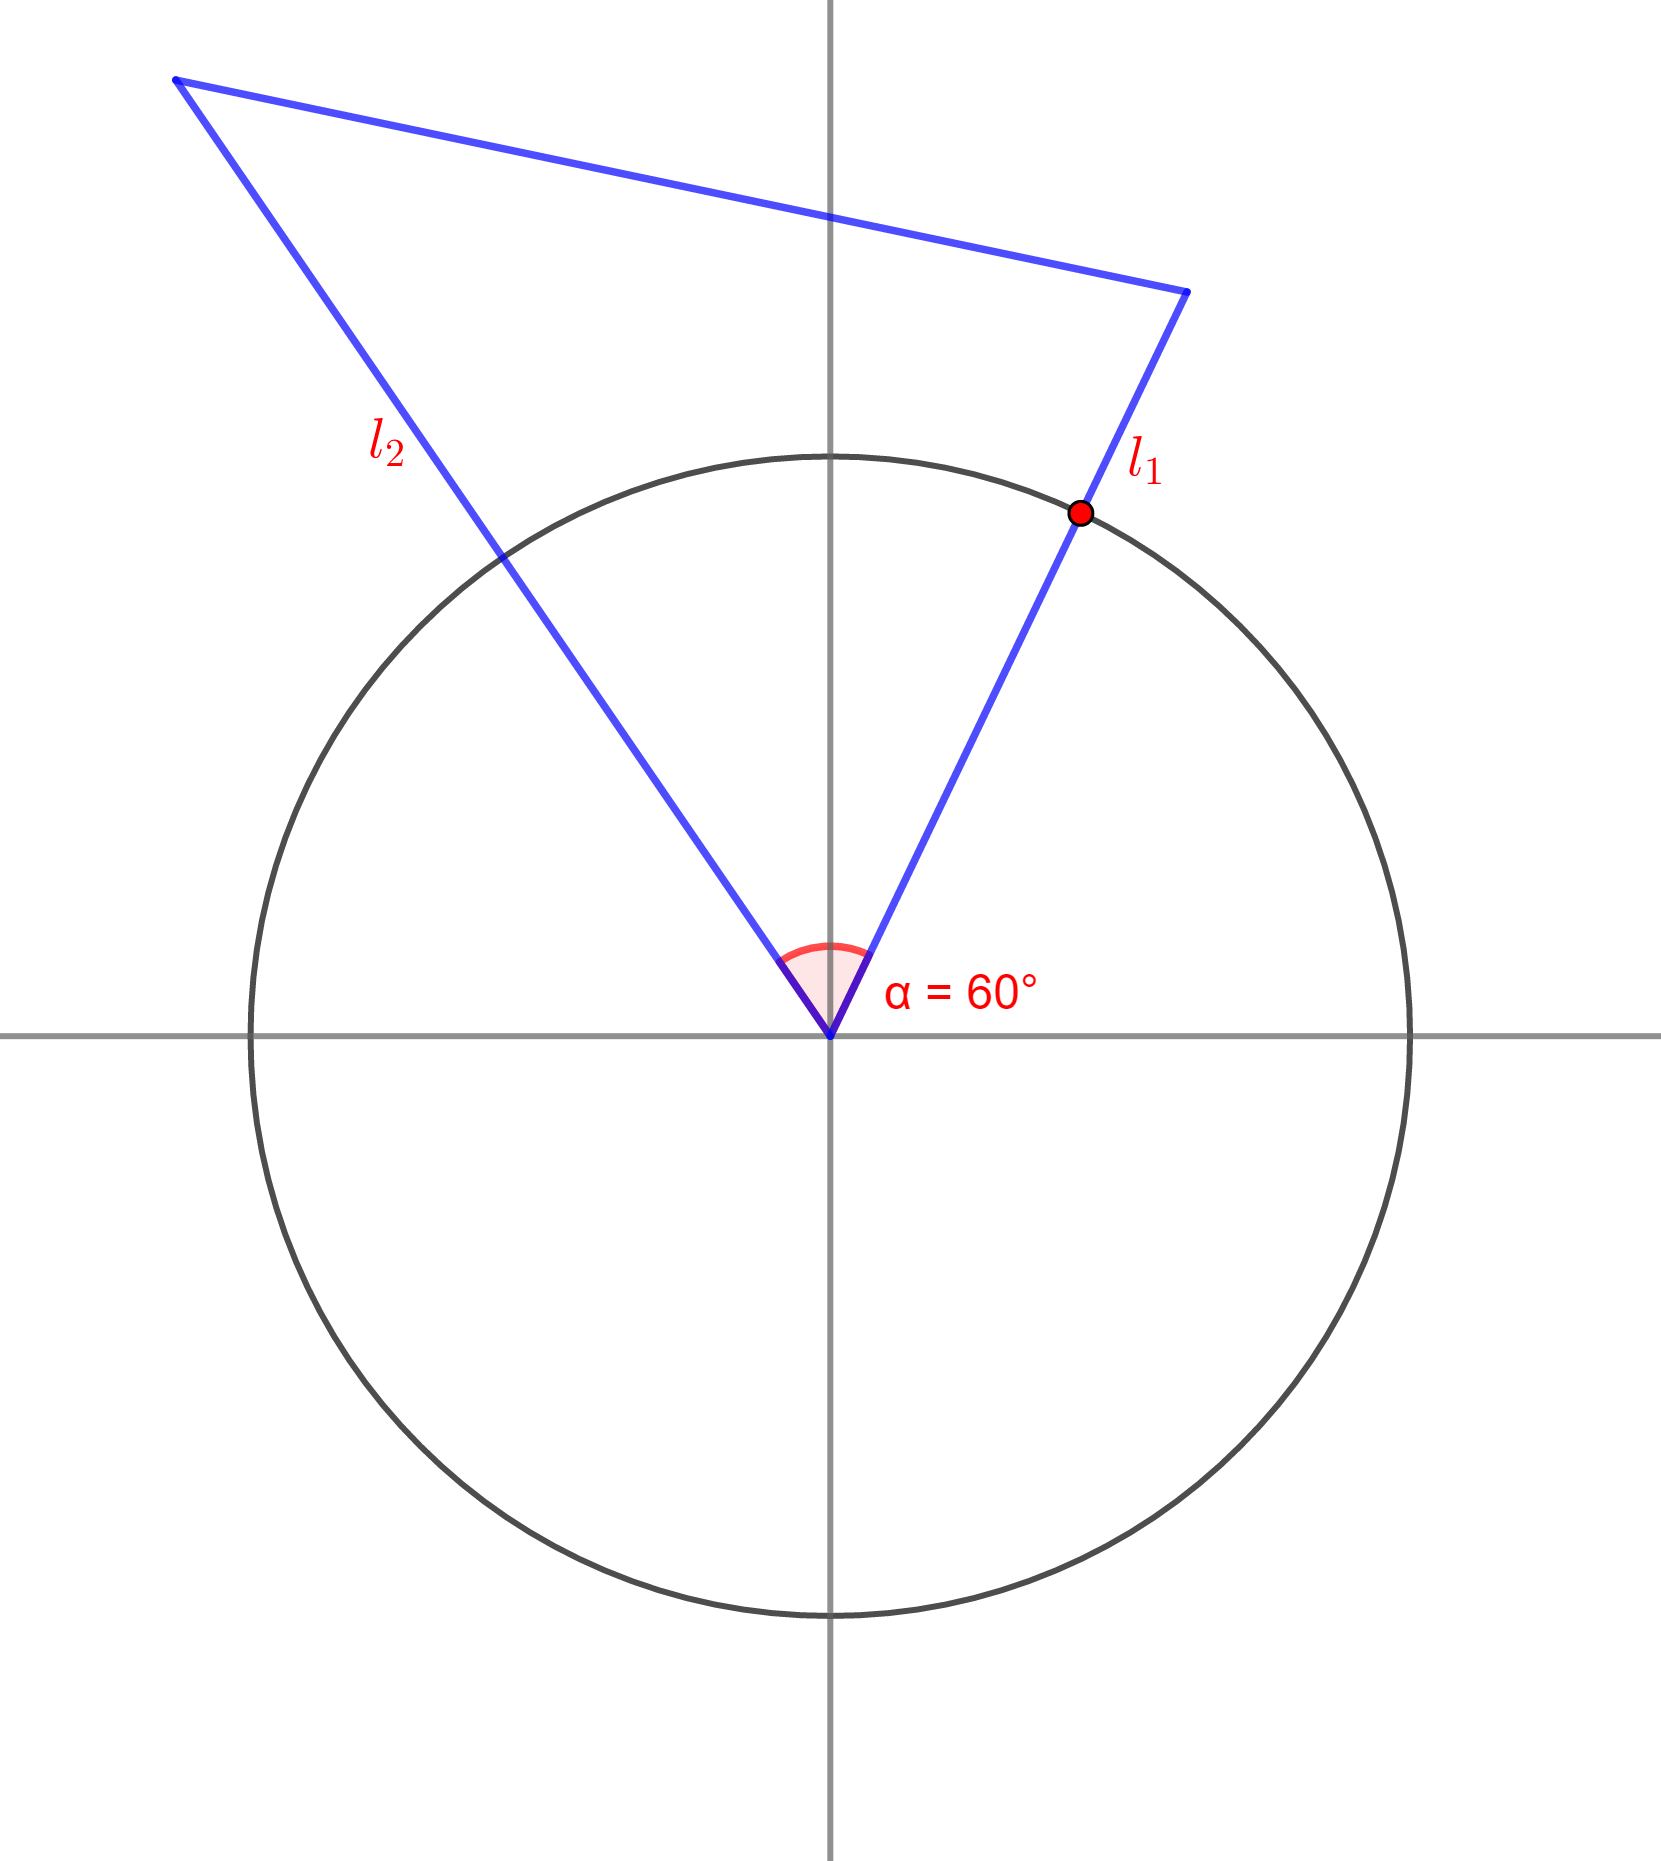
\includegraphics[width=0.6\linewidth]{Pic2}
	\end{figure}\\
	Тогда 
	\begin{gather*}
		\int I_{A_i} d\mu_1 = \lim\limits_{n \to \infty} \int_x f_n d \mu_1
	\end{gather*}
	Так как $f_i$ непрерывна и ограничена, то
	\begin{gather*}
		\lim\limits_{n \to \infty} \int_x f_n d \mu_1 = \lim\limits_{n \to \infty} \int_x f_n d \mu_2 = \int I_{A_i} d \mu_2\\
		\int I_{A_i} (x) d\mu_1 = \int I_{A_i}(x) d\mu_2
	\end{gather*}